\section{Nation-State Routing: State of the Art -- \annie{this section needs a better name to describe the initial measurements we did from probes to the Top 100 domains}}
\label{measure}

As Internet traffic crosses international borders, it becomes subject to the wiretapping policies of the national jurisdiction in which it is transitting.  Some countries, such as the United States, are well known for wiretapping policies.  The methods we use are general and can be applied to any country of interest, and we describe our measurement pipeline for Country X. We measure where Country X's Internet users' traffic is going and how often; this shows how much possible surveillance could currently be conducted on Country X's traffic.  We then apply our measurements to Brazil, Netherlands, India, Kenya, and the United States and discuss the results.

\subsection{Brazil}
Here we discuss our findings on which countries transit Brazilian web traffic, which countries host popular content for Brazilians, and to which countries Brazilian traffic trombones.  

\begin{figure}
\centering
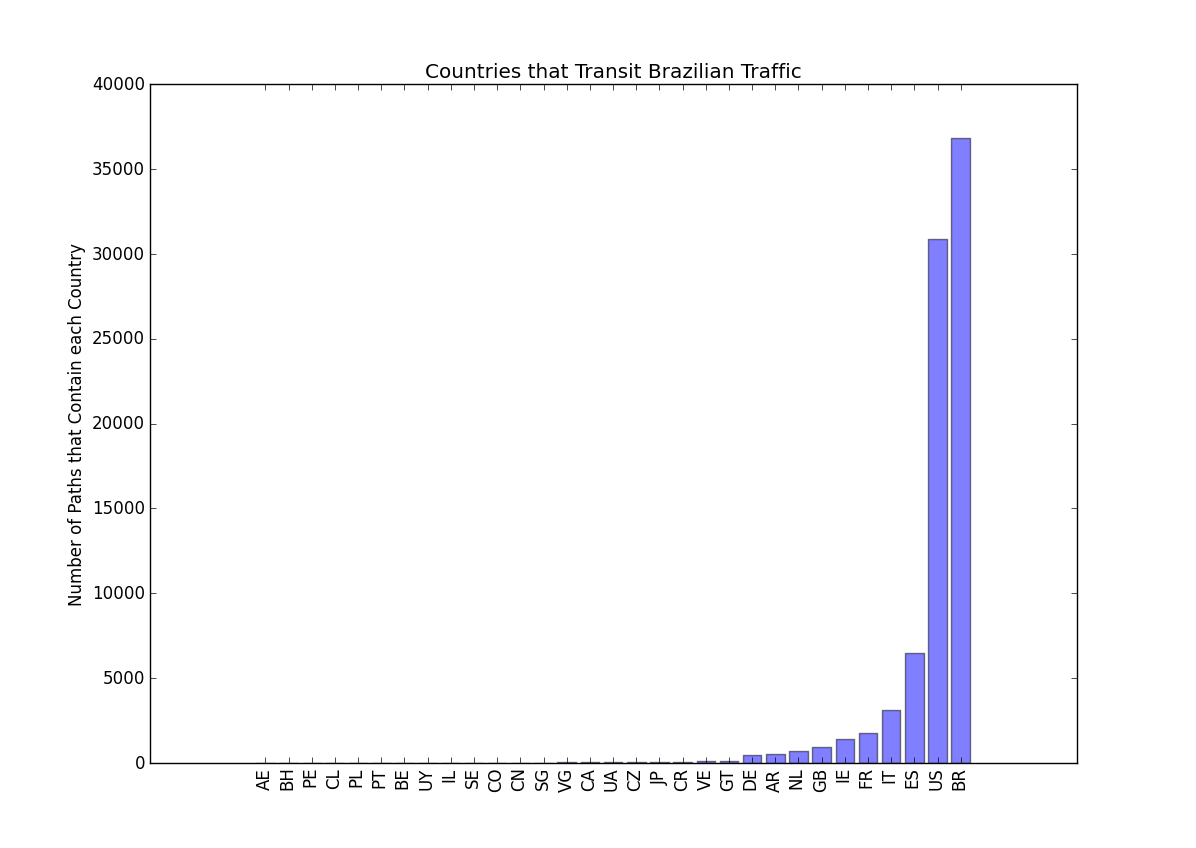
\includegraphics[width=.5\textwidth]{br_transit_bar}
\caption{The number of paths that Brazilian traffic transits.}
\label{fig:transit_br}
\end{figure}

Figure \ref{fig:transit_br} shows the number of paths that transit different countries.  Note that these numbers are calculated for when the country is \textit{only} on the path and \textit{not the destination country}.  We can see that Brazil is most commonly on the path, which is expected because all paths originate from Brazil.  A few countries see a significant amount of traffic; Spain transits 17.6\% of the paths, Italy transits 8.4\% of the paths, and the United States transits 7.3\% of the paths.  Any country that is on the path has the ability to conduct surveillance on Brazilian traffic.  

More revealing than the transit-only countries, the paths that end in countries other than Brazil show that web content for Brazilian Internet users is not primarily hosted in Brazil.  The number of paths that end in different countries are shown in Figure \ref{fig:host_br}.  The country that hosts the most significant amount of web content is the United States; it was the destination country for 77\% of paths from Brazil.  If most of these domains are only hosted in the United States, then it's impossible for Brazilian clients to avoid the United States.  If the web content is georeplicated in another region, such as Europe, then Brazilian clients may be able to avoid the United States for a significant amout of their Internet traffic.  It is also worth noting that only 17\% of the paths end in Brazil, and the next most popular destination country is Ireland with 1.7\% of paths ending there.  

Tromboning paths show that local traffic isn't staying local; ideally, if a path starts and ends in the same country, then it shouldn't cross international borders.  We found that tromboning occurs for Brazilian traffic to 9 different countries.  These results can be seen in Figure \ref{fig:trombone_br}.  While we measured 4.2\% of all paths trombone, 81\% of all tromboning paths go through the United States.  For 4.2\% of the traffic, foreign countries can conduct surveillance because the traffic is not staying local (but should be). 

\begin{figure}[t!]
\centering
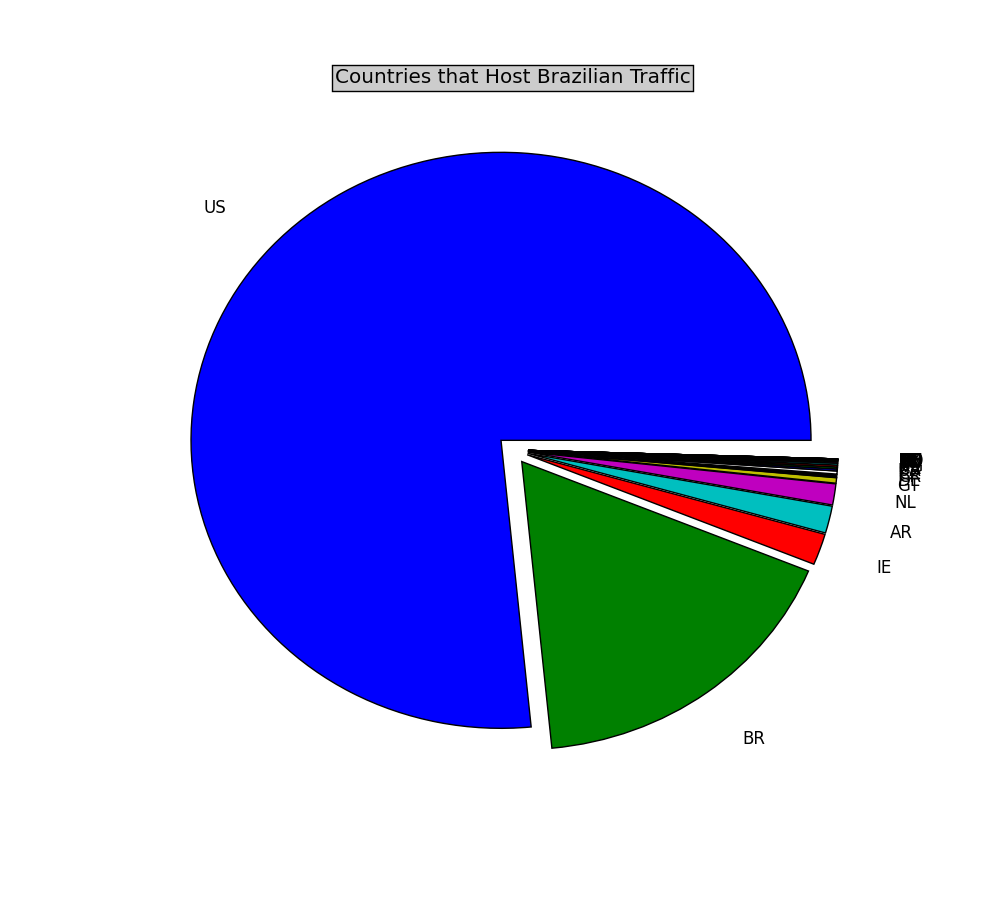
\includegraphics[width=.5\textwidth]{brazil_host}
\caption{The number of paths that end in a country.}
\label{fig:host_br}
\end{figure} 

\begin{figure}
\centering
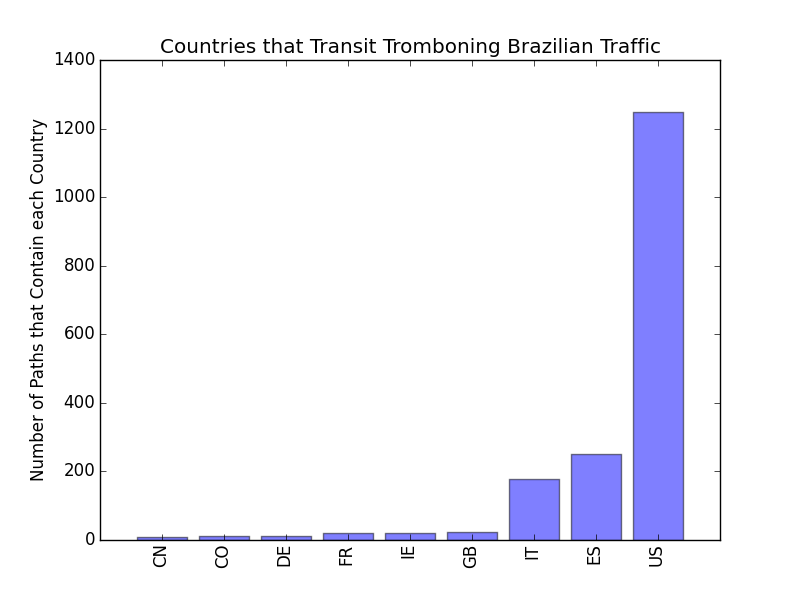
\includegraphics[width=.5\textwidth]{br_trombone}
\caption{The number of paths that start and end in Brazil, but pass through another country.}
\label{fig:trombone_br}
\end{figure}

These results show that there are numerous opportunities for foreign countries to conduct surveillance on Brazilian citizens because of interdomain routing. 

\subsection{Netherlands}
Here we discuss our results for which countries route and/or host Netherlands traffic. 

Similar to the findings about Brazil, the United States is the foreign country that transits {\it and} hosts the Netherlands traffic most often.  Transit countries and hosting countries for traffic generated by clients in the Netherlands are shown in Figures \ref{fig:transit_nl} and \ref{fig:host_nl}.  Most other countries that transit Netherlands traffic are European countries, such as Great Britain, Ireland, France, Sweden, and Germany.

\begin{figure}
\centering
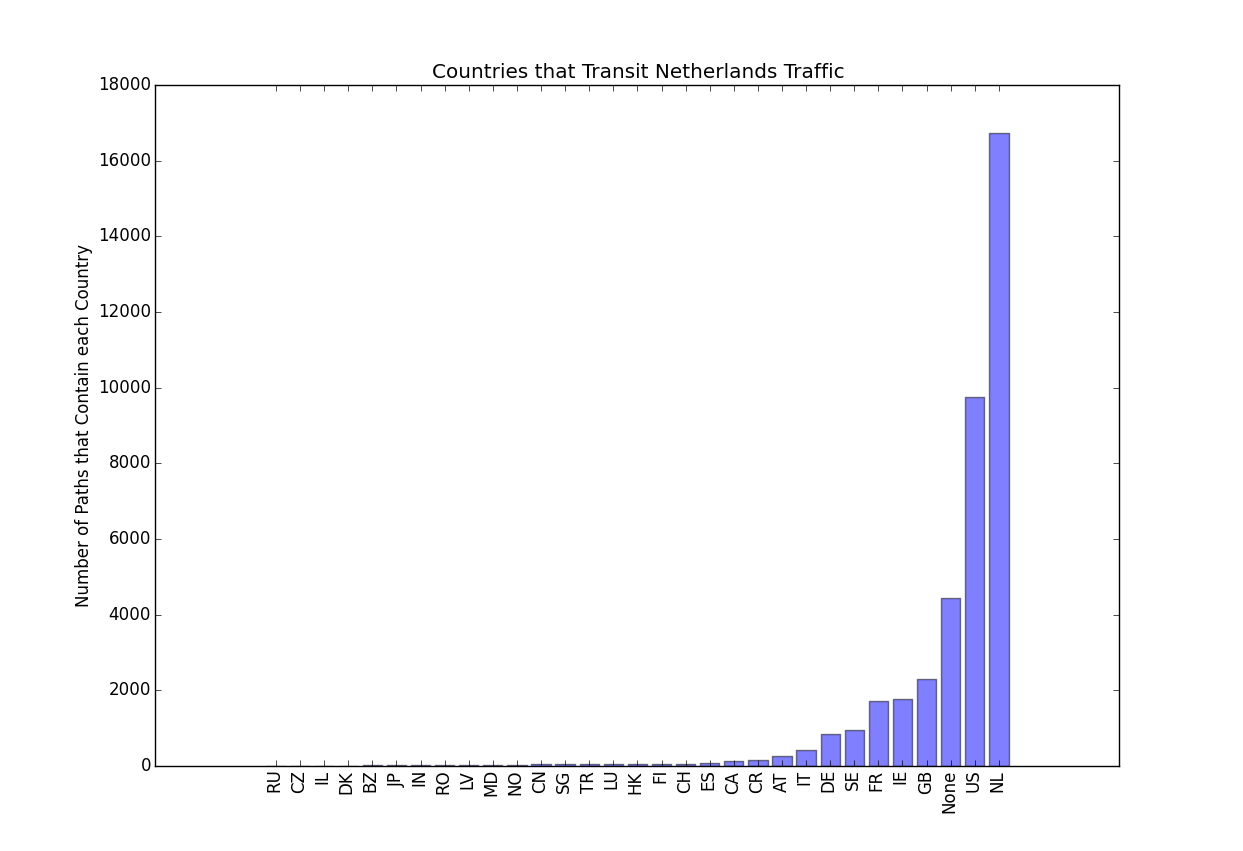
\includegraphics[width=.5\textwidth]{nl_transit_nl}
\caption{The number of paths that Netherlands traffic transits.}
\label{fig:transit_nl}
\end{figure}

\begin{figure}[t!]
\centering
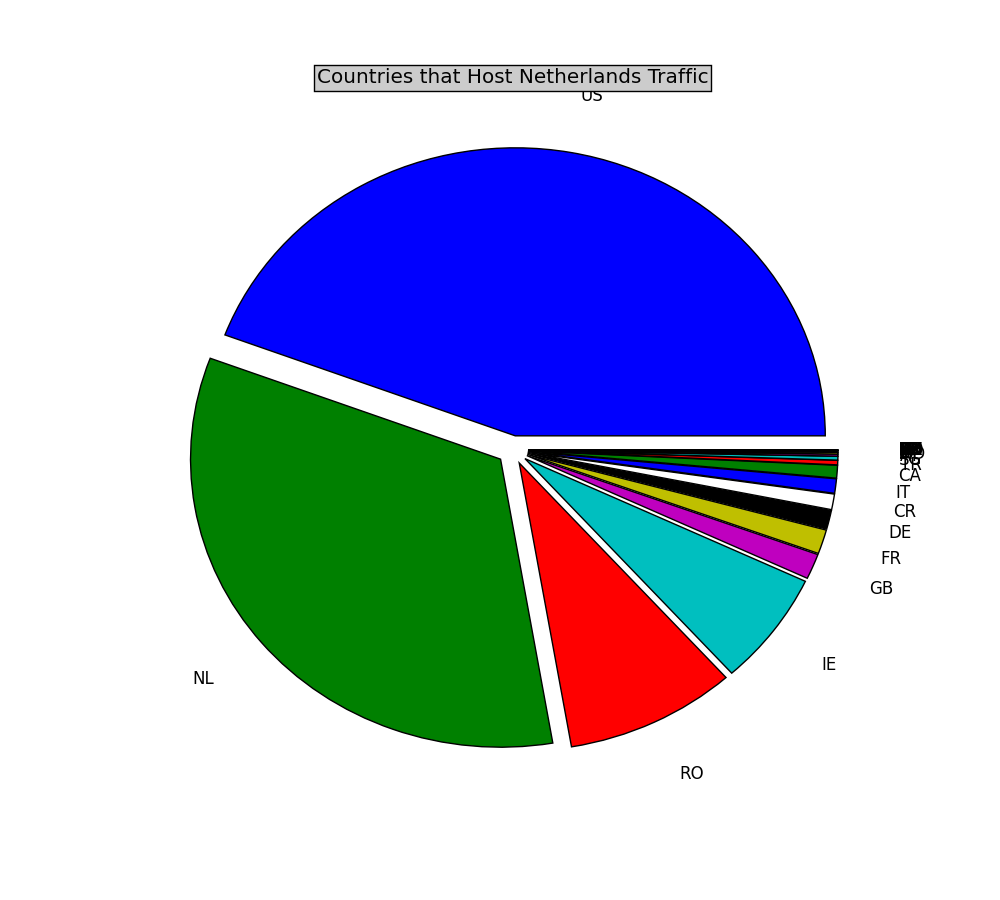
\includegraphics[width=.5\textwidth]{netherlands_host}
\caption{The number of paths that end in a country.}
\label{fig:host_nl}
\end{figure} 

The percentage of popular domains that are hosted in the Netherlands is similar to the percentage that are hosted in the United States.  Like the transit countries, most of the other countries that host popular domains are in other European countries.

About a third (33.4\%) of the Netherlands traffic in our study was domestic traffic, and about half (52.2\%) of the domestic traffic tromboned to countries other than the Netherlands.  The United States and Great Britain saw the most of the Netherlands tromboning domestic traffic --- both of which are known for surveillance.

\begin{figure}
\centering
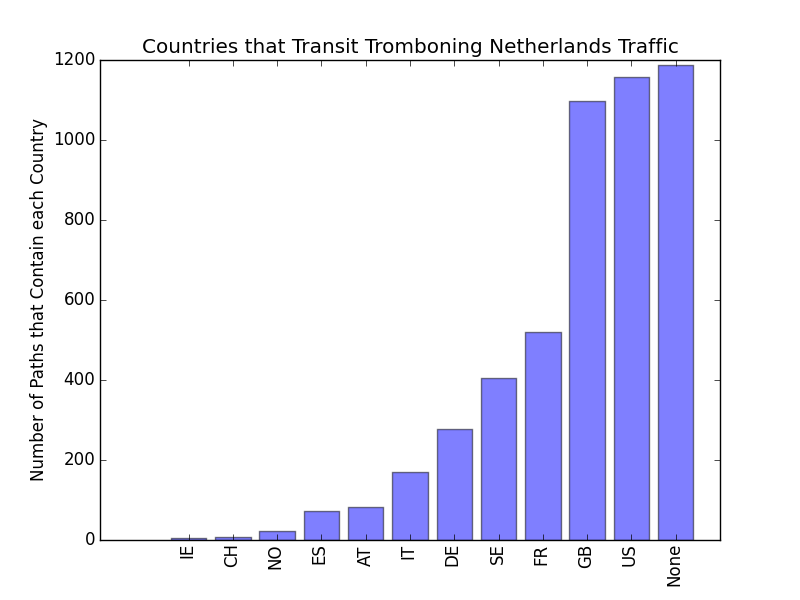
\includegraphics[width=.5\textwidth]{nl_trombone}
\caption{The number of paths that start and end in Netherlands, but pass through another country.}
\label{fig:trombone_nl}
\end{figure}

\subsection{India}
\annie{add India results here}

\begin{figure}
\centering
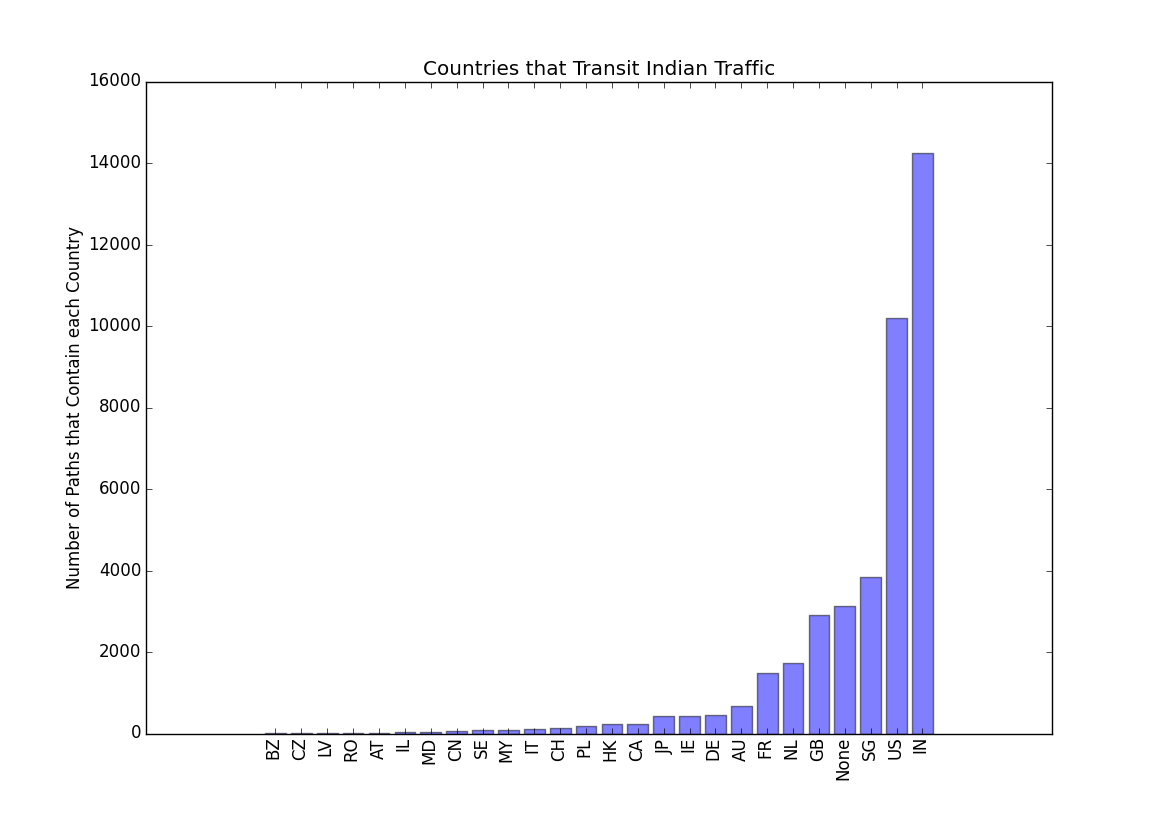
\includegraphics[width=.5\textwidth]{in_transit_bar}
\caption{The number of paths that Indian traffic transits.}
\label{fig:transit_in}
\end{figure}

\begin{figure}[t!]
\centering
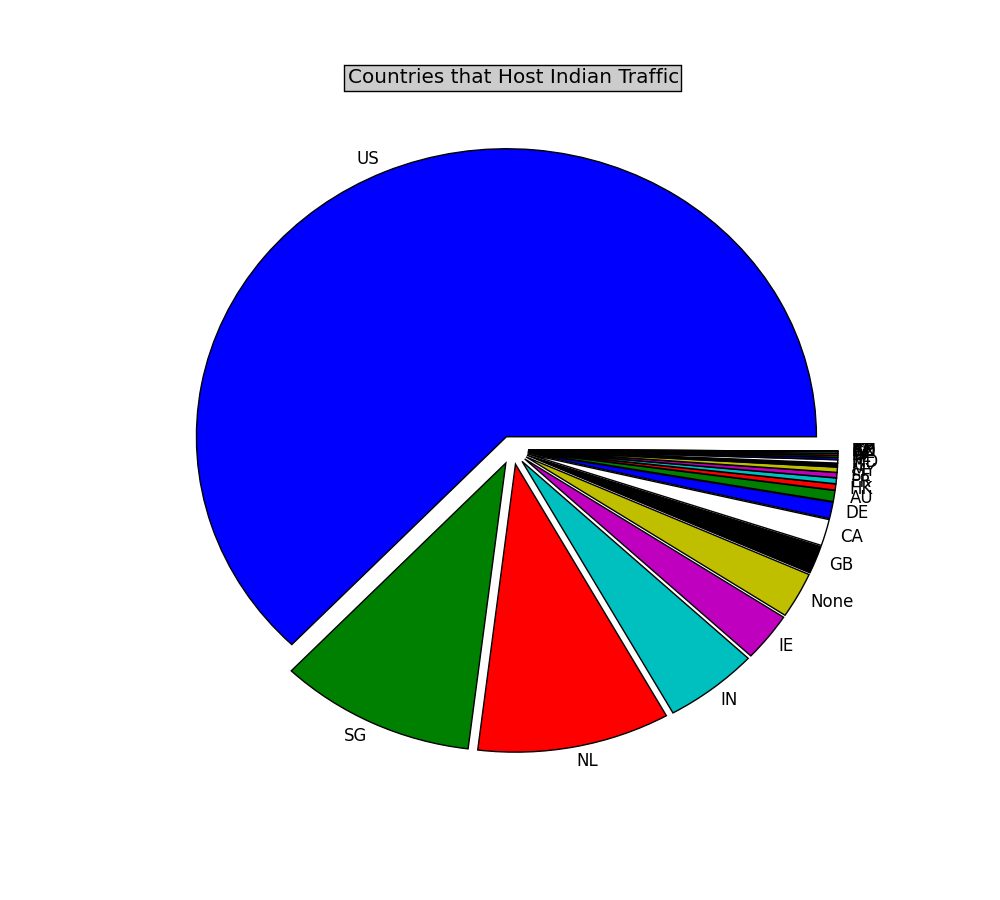
\includegraphics[width=.5\textwidth]{india_host}
\caption{The number of paths that end in a country.}
\label{fig:host_in}
\end{figure} 

\begin{figure}
\centering
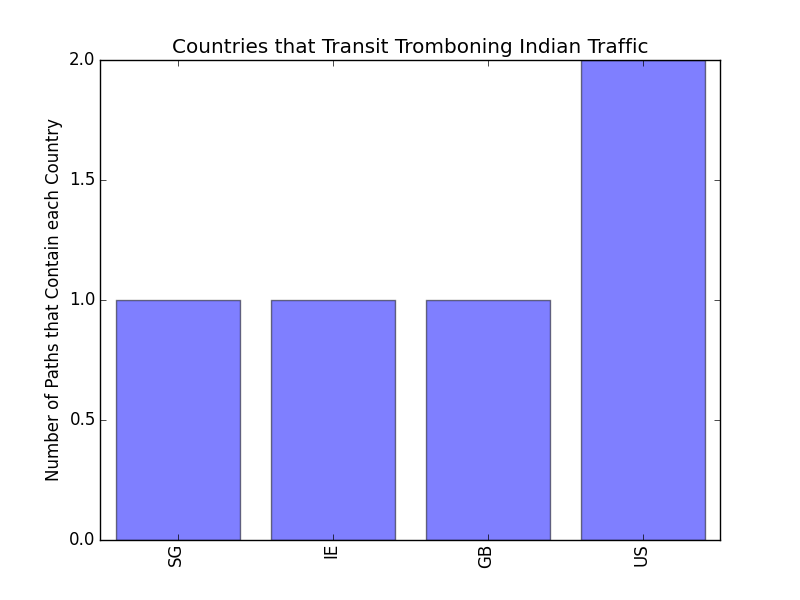
\includegraphics[width=.5\textwidth]{in_trombone}
\caption{The number of paths that start and end in India, but pass through another country.}
\label{fig:trombone_in}
\end{figure}

\subsection{Kenya}
\annie{add Kenya results here}

\begin{figure}
\centering
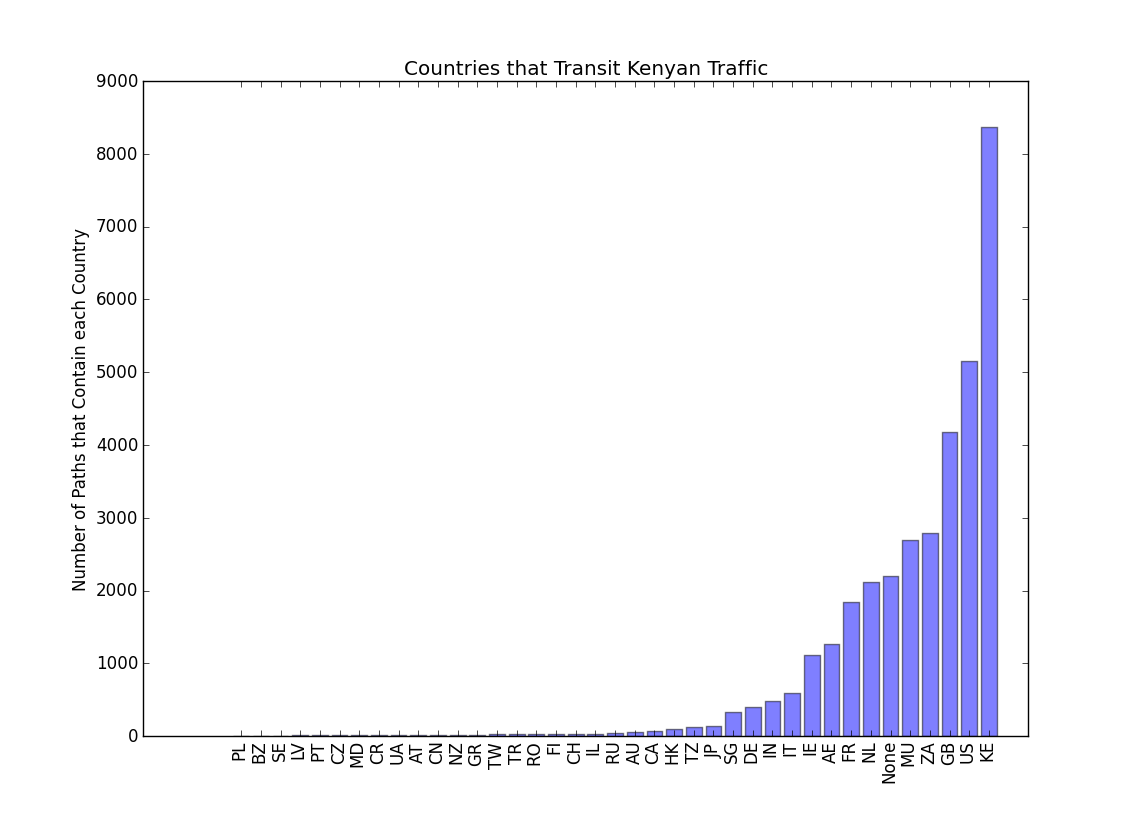
\includegraphics[width=.5\textwidth]{ke_tranit_bar}
\caption{The number of paths that Kenyan traffic transits.}
\label{fig:transit_ke}
\end{figure}

\begin{figure}[t!]
\centering
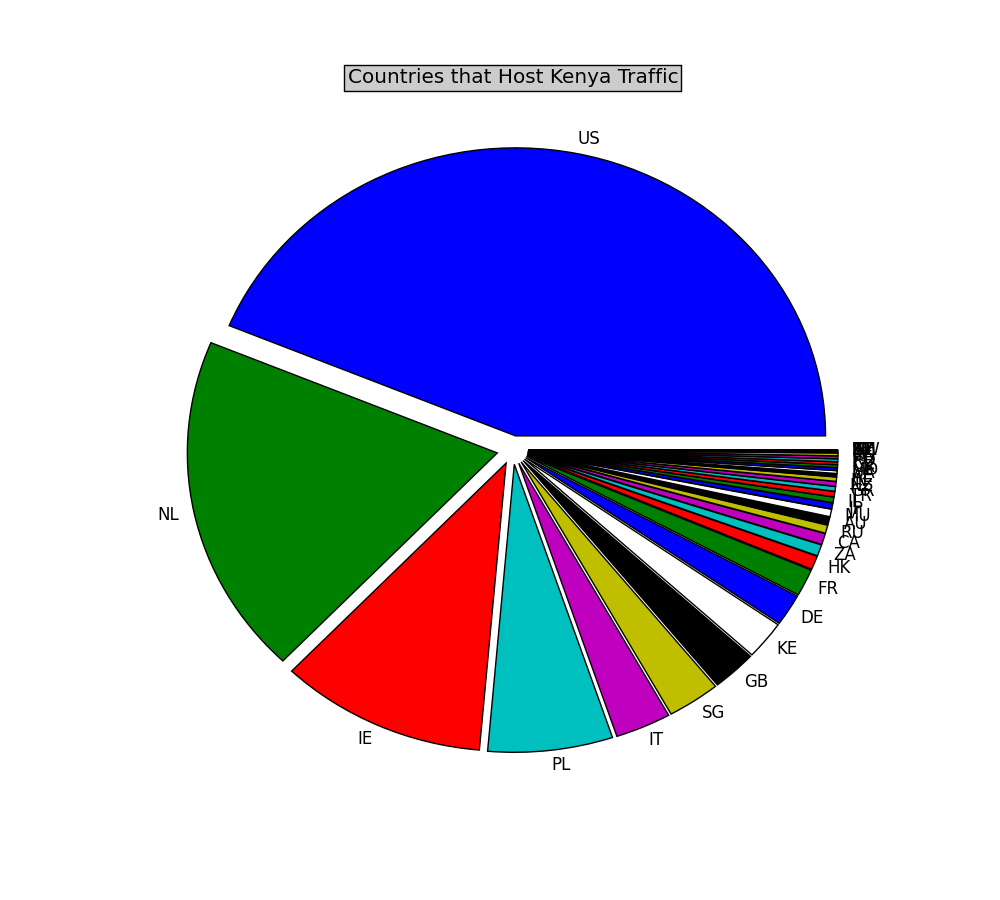
\includegraphics[width=.5\textwidth]{kenya_host}
\caption{The number of paths that end in a country.}
\label{fig:host_ke}
\end{figure} 

\begin{figure}
\centering
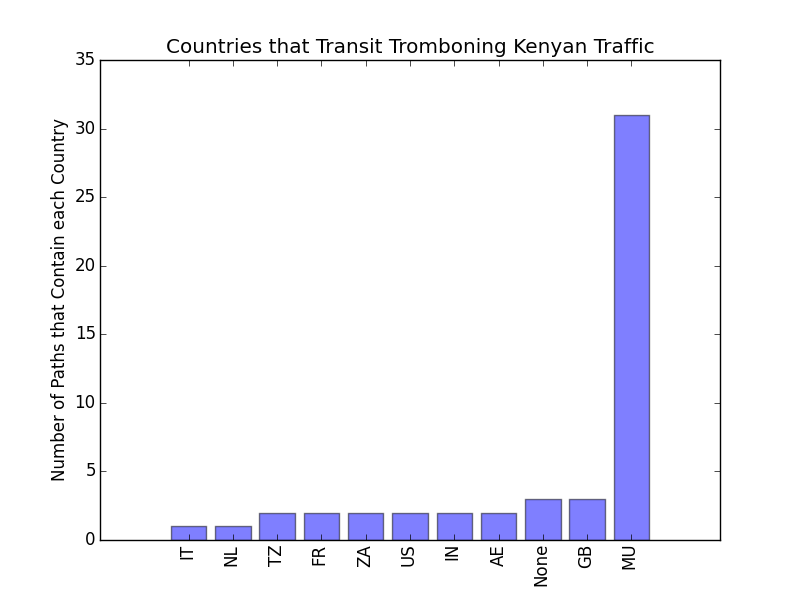
\includegraphics[width=.5\textwidth]{ke_trombone}
\caption{The number of paths that start and end in Kenya, but pass through another country.}
\label{fig:trombone_ke}
\end{figure}

\subsection{United States}

\begin{figure}
\centering
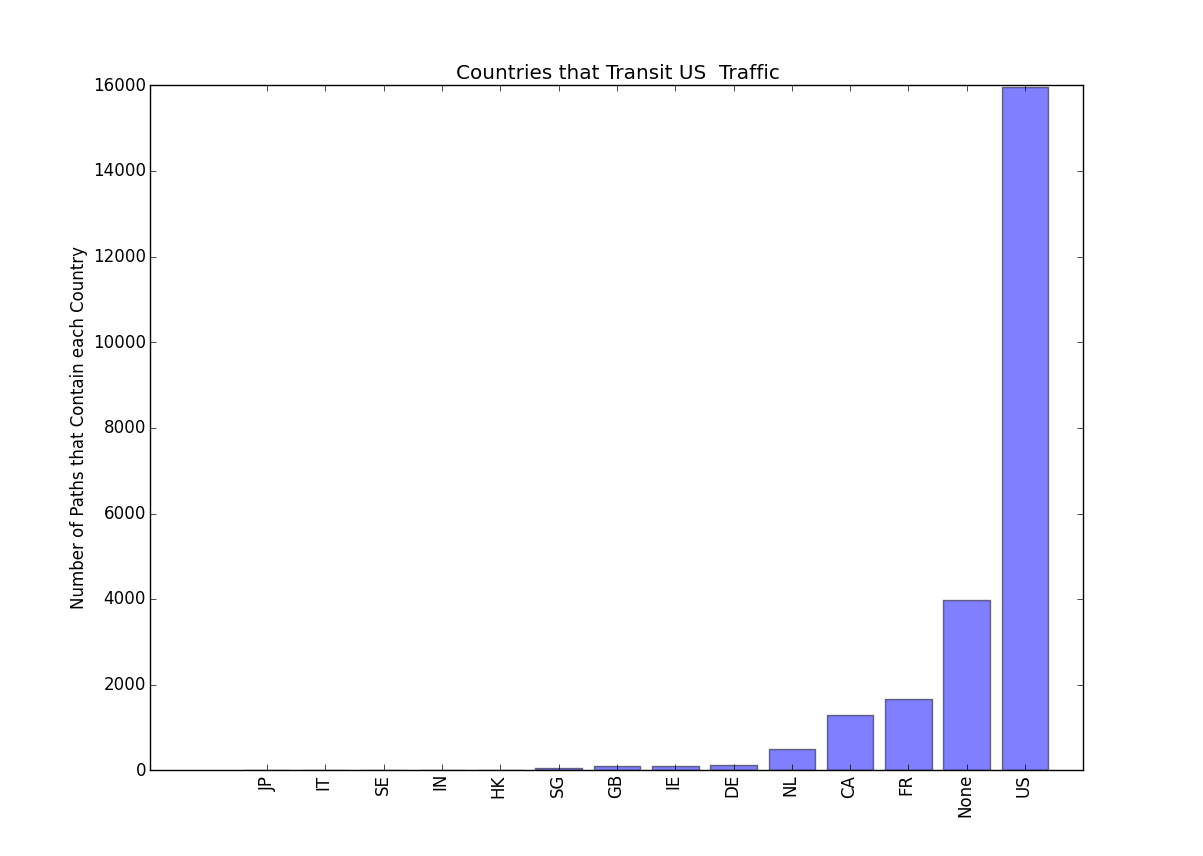
\includegraphics[width=.5\textwidth]{us_transit_bar}
\caption{The number of paths that United States traffic transits.}
\label{fig:transit_us}
\end{figure}

\begin{figure}[t!]
\centering
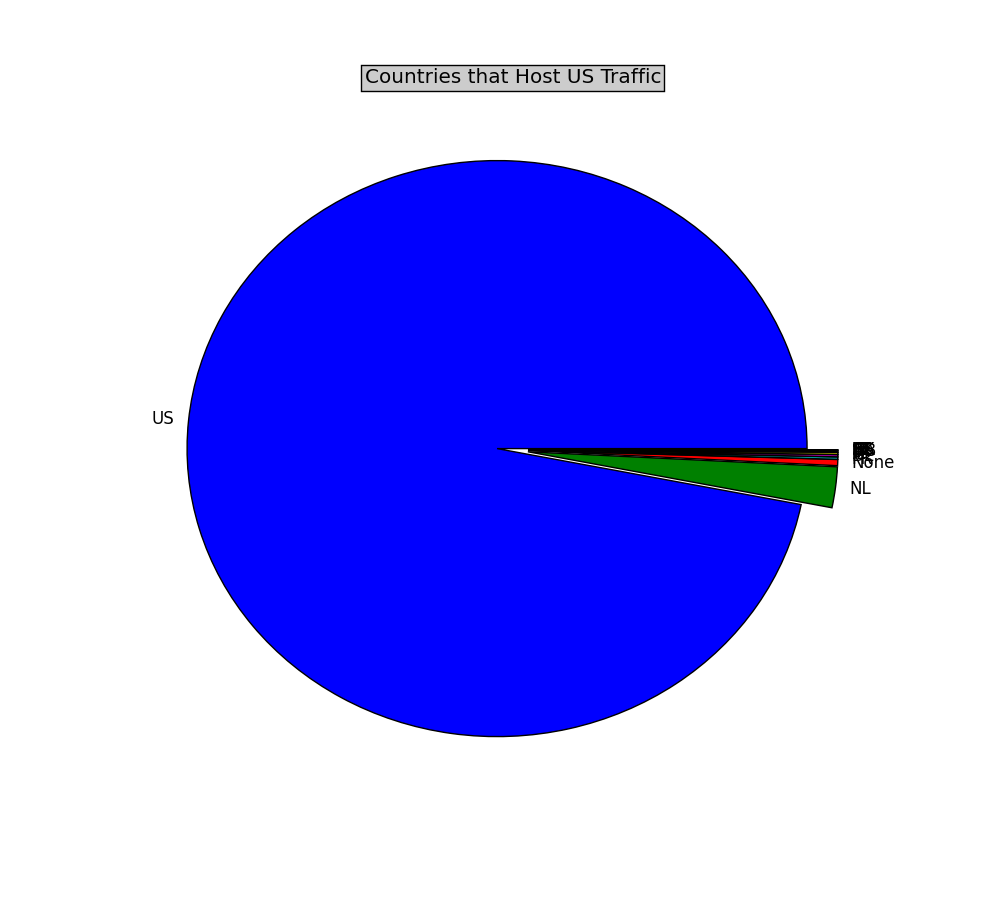
\includegraphics[width=.5\textwidth]{us_host}
\caption{The number of paths that end in a country.}
\label{fig:host_us}
\end{figure} 

\begin{figure}
\centering
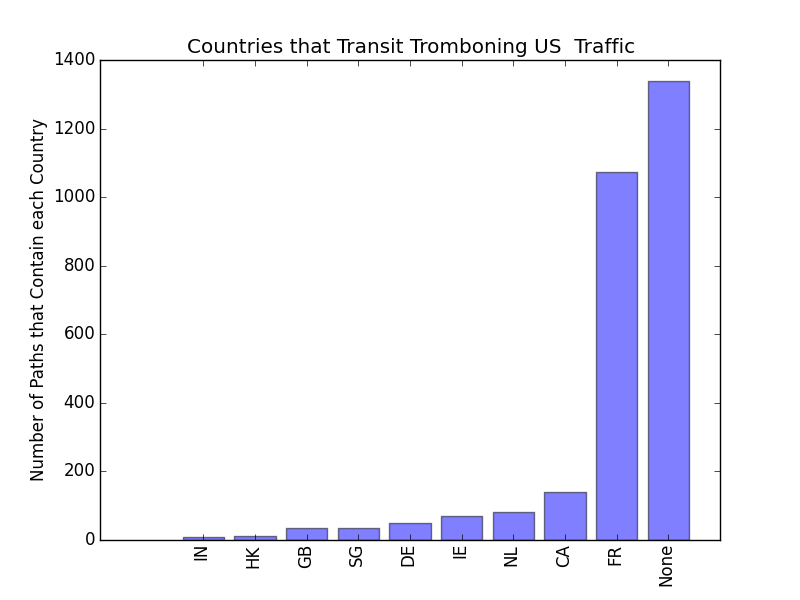
\includegraphics[width=.5\textwidth]{us_trombone}
\caption{The number of paths that start and end in United States, but pass through another country.}
\label{fig:trombone_us}
\end{figure}
